
%%%%%%%%%%%%%%%%%%%%%%%%%%%%%%%%%%%%%%%%%
% Journal Article
% LaTeX Template
% Version 2.0 (February 7, 2023)
%
% This template originates from:
% https://www.LaTeXTemplates.com
%
% Author:
% Vel (vel@latextemplates.com)
%
% License:
% CC BY-NC-SA 4.0 (https://creativecommons.org/licenses/by-nc-sa/4.0/)
%
% NOTE: The bibliography needs to be compiled using the biber engine.
%
%%%%%%%%%%%%%%%%%%%%%%%%%%%%%%%%%%%%%%%%%

%----------------------------------------------------------------------------------------
%	PACKAGES AND OTHER DOCUMENT CONFIGURATIONS
%----------------------------------------------------------------------------------------

\documentclass[
	a4paper, % Paper size, use either a4paper or letterpaper
	12pt, % Default font size, can also use 11pt or 12pt, although this is not recommended
	unnumberedsections, % Comment to enable section numbering
	twoside, % Two side traditional mode where headers and footers change between odd and even pages, comment this option to make them fixed
]{LTJournalArticle}

% \runninghead{Jurnal - 1313618030 - Farhan Herdian Pradana } % A shortened article title to appear in the running head, leave this command empty for no running head

% \footertext{\textit{Journal of Biological Sampling} (2024) 12:533-684} % Text to appear in the footer, leave this command empty for no footer text

%equation
\usepackage{amsmath}
\allowdisplaybreaks

%algoritma
\usepackage{algorithm}
\usepackage{algpseudocode}

\makeatletter
\newenvironment{breakablealgorithm}
{
    \begin{center}
        \refstepcounter{algorithm}
        \renewcommand{\caption}[1]
        {
            \addcontentsline{loa}{algorithm}{\protect\numberline{\thealgorithm}##1}
            \parbox{\textwidth}
            % Makes a unbreakable block and can also be done by `minipage`.
            {
                \hrule height.8pt depth0pt \kern2pt
                {\raggedright\textbf{\fname@algorithm~\thealgorithm} ##1\par}
                \kern2pt\hrule\kern2pt
            }
        }
}
{
        \kern2pt\hrule\relax
    \end{center}
}
\makeatother

\usepackage{longtable}

\setcounter{page}{1} % The page number of the first page, set this to a higher number if the article is to be part of an issue or larger work

%----------------------------------------------------------------------------------------
%	TITLE SECTION
%----------------------------------------------------------------------------------------

\title{Perbandingan Implementasi Algoritma-algoritma Pagerank pada Satu Mesin Komputer} % Article title, use manual lines breaks (\\) to beautify the layout

% Authors are listed in a comma-separated list with superscript numbers indicating affiliations
% \thanks{} is used for any text that should be placed in a footnote on the first page, such as the corresponding author's email, journal acceptance dates, a copyright/license notice, keywords, etc
\author{%
	Farhan Herdian Pradana\textsuperscript{1}, Muhammad Eka Suryana\textsuperscript{2}, Med Irzal\textsuperscript{3}
}

% Affiliations are output in the \date{} command
\date{
	\footnotesize
	Program Studi Ilmu Komputer, Fakultas Matematika dan Ilmu Pengetahuan Alam \\
	Universitas Negeri Jakarta, DKI Jakarta, Indonesia \\
	\textsuperscript{\textbf{1}}farhan.herdia123@gmail.com, 
	\textsuperscript{\textbf{2}}eka-suryana@unj.ac.id, 
	\textsuperscript{\textbf{3}}medirzal@unj.ac.id
}

% Full-width abstract
\renewcommand{\abstractname}{Abstrak}
\renewcommand{\maketitlehookd}{%
	\begin{abstract}
		\noindent Algoritma Pagerank merupakan algoritma mengurutkan halaman web pada \textit{search engine} Google. Masalah pada Algoritma Pagerank adalah memerlukan memori utama yang cukup besar, dan tidak mungkin dilakukan pada satu mesin komputer dengan memori utama yang terbatas. Akan dicari algoritma alternatif dari Algoritma Pagerank Original buatan Google dengan membandingkannya pada algoritma-algoritma Pagerank dari penelitian lainnya dengan membandingkan kecepatan, penggunaan memori utama, dan kemiripan hasil. Penelitian dilakukan dengan melakukan pengkodean terhadap algoritma Pagerank Original, algoritma Distributed Pagerank Computation (DPC), algoritma Modified DPC (MDPC), dan algoritma Random Walker. Semua kode program dijalankan pada dataset dan dibandingkan kecepatan, penggunaan memori utama, dan kemiripan hasil akhirnya. Khusus hasil akhir, hasil dari algoritma Random Walker dijadikan acuan karena dasar dari Algoritma Pagerank adalah Random Walker. Hasilnya Algoritma Pagerank Original unggul dari sisi kecepatan dan hasil yang mirip dengan hasil Algoritma Random Walker. Sedangkan algoritma DPC dan MDPC unggul di penggunaan memori utama yang lebih hemat, sehingga cocok untuk satu mesin komputer yang memiliki memori utama yang terbatas, tetapi dengan catatan mengorbankan kecepatan yang lebih lambat dan hasil yang tidak mirip terhadap Random Walker.
	\end{abstract}
}

%----------------------------------------------------------------------------------------

\begin{document}

\maketitle % Output the title section

%----------------------------------------------------------------------------------------
%	ARTICLE CONTENTS
%----------------------------------------------------------------------------------------

\section{I. PENDAHULUAN}

Internet adalah jaringan luas yang membuat jaringan komputer seluruh dunia dapat saling berkomunikasi \citep{sample2018internet}. Internet melahirkan World Wide Web (WWW) yang memungkinkan situs web atau biasa disebut \textit{website} untuk bisa diakses oleh semua orang. \textit{Website} adalah sekumpulan halaman web yang saling terkait dan berada pada nama domain yang sama. Website dapat dibuat dan dipelihara oleh seorang individu, grup, perusahaan, atau organisasi lain dengan berbagai macam tujuan \citep{techopedia2020website}. Pada tahun 1992 hanya terdapat sepuluh \textit{website}, lalu pada tahun 1994 angka ini bertumbuh menjadi 3.000 \textit{website}, dan semakin bertumbuh pesat pada tahun 2021 menjadi kurang lebih 1,88 miliar \textit{website} \citep{amstrong2021website}.

Dengan meledaknya jumlah halaman web, memunculkan tantangan baru dalam memperoleh informasi dari web. Pengguna biasanya menelusuri web dengan mengunjungi graf \textit{link} yang terdapat pada halaman web, biasanya dimulai pada situs kumpulan index halaman web berkualitas tinggi yang dipelihara oleh manusia seperti Yahoo.com, atau menggunakan \textit{search engine} \citep{brin1998anatomy}. Seiring perkembangan zaman, \textit{search engine} Google menjadi \textit{search engine} teratas dengan pengguna terbesar di dunia dengan penguasaan pasar sebesar 91\% \citep{gsc2022marketshare}. Kunci kesuksesan dari Google terletak pada Pagerank. Pagerank merangking halaman web berdasarkan kepentingan relatif (\textit{relative importance}) suatu halaman web berdasarkan graf tautan web \citep{ilprints422}. 

Dalam melakukan perangkingan halaman web, Pagerank dapat didefinisikan pada persamaan \ref{eq:1}. Dimana $u$ adalah halaman web. $F_u$ adalah himpunan halaman $u$ yang menunjuk halaman lain dan $B_u$ adalah himpunan halaman yang menunjuk ke $u$. $C_u = |F_u|$ adalah jumlah \textit{link} dari $u$ dan $c$ adalah faktor yang digunakan untuk normalisasi (sehingga jumlah total \textit{ranking} semua halaman web adalah konstan) dan $c < 1$. $E(u)$ adalah vektor yang berkorespondensi dengan \textit{ranking} halaman web. $||\pi'||_1 = 1$. Iterasi perhitungan terus dilakukan sampai konvergen. Jika diubah kedalam persamaan matriks, maka persamaan \ref{eq:1} dapat diubah menjadi persamaan \ref{eq:2}. Dimana $X$ adalah matriks persegi yang baris dan kolomnya berkorespondensi dengan halaman web, dengan elemen $X_{u,v} = \frac{1}{C_u}$ jika terdapat \textit{link} pada halaman $u$ ke halaman $v$ atau $X_{u,v} = 0$ jika tidak ada.

\begin{equation}
	\label{eq:1}
	\pi'(u) = c\sum_{v\in B_u} \frac{\pi'(v)}{C_v} + cE(u)
\end{equation}

\begin{equation}
	\label{eq:2}
	\pi'=c(X\pi' + E)
\end{equation}

Dasar intuitif dari persamaan \ref{eq:1} adalah \textit{random walks} pada sebuah graf. Anggap pengguna internet sebagai \textit{"random surfer"} yang terus meng-klik \textit{link} selanjutnya secara acak. Namun, jika pengguna terjebak pada sebuah lingkaran halaman web (\textit{link} yang diklik terus menampilkan halaman web yang pernah dikunjungi sebelumnya), tidak mungkin pengguna akan terus mengikuti \textit{link} tersebut, melainkan pengguna akan langsung pindah ke halaman lain. Oleh sebab itu faktor $E$ dipakai untuk memodelkan perilaku ini (Pengguna akan bosan dan langsung lompat ke halaman web lain berdasarkan distribusi pada $E$) \citep{ilprints422}. $E$ dapat didefinisikan oleh pengguna (\textit{user-defined parameter}) dan nilai elemennya dapat diisi dengan nilai yang seragam atau berbeda-beda. Menariknya, jika nilai elemen $E$ dibuat berbeda-beda, maka dapat membuat Pagerank yang dipersonalisasi \citep{ilprints422}.

Walaupun persamaan Pagerank terlihat sederhana, terdapat masalah dari sisi ruang dan waktu. Dari sisi ruang, misal terdapat 1000 halaman web, maka akan terbentuk 1000x1000 matriks $X$. Misal tiap sel elemen $X$ memerlukan memori 8 \textit{Byte}, maka untuk membentuk 1000x1000 matriks $X$, tanpa menghitung alokasi \textit{overhead} memori, memerlukan 8 \textit{Mega Byte} (MB) memori utama (Lihat tabel \ref{table:1}). Di internet terdapat miliaran \textit{website} dan setiap \textit{website} dapat memiliki lebih dari 1 halaman, sehingga untuk bisa membentuk matriks $X$ membutuhkan memori utama dengan kapasitas mencapai \textit{Peta Byte} atau bahkan \textit{Exa Byte}. Hal tersebut sangat tidak mungkin dilakukan pada komputer pribadi biasa yang memori utamanya hanya pada kisaran 4 GB sampai 32 GB, yang berarti ketika program dieksekusi langsung \textit{crash} karena memori yang tidak cukup. Dari sisi waktu, proses \textit{string matching} untuk mengakses nilai \textit{ranking} suatu halaman web berdasarkan \textit{string} URLnya juga memiliki kompleksitas waktu yang besar yakni O(NM), jika dilakukan dengan cara dicari satu-persatu. Beruntung \textit{database} seperti MySQL menggunakan B-Tree dalam mengindeks datanya \citep{mysqlIndex}. B-tree memiliki kompleksitas waktu kecil yakni hanya O(log(n)) \citep{geeksForGeeksBtree}.


\begin{table}
	\centering
	\caption{Tabel alokasi memori utama untuk membentuk matriks $X$}
	\label{table:1}
	\begin{tabular}{|c|c|} 
		\hline
		Jumlah Halaman Web & Memori (\textit{Byte}) \\
		\hline
		
		\hline
		256 & 524416 \\
		512 & 2097280 \\
		1024 & 8388736 \\
		2048 & 33554560 \\
		4096 & 134217856 \\
		8192 & 536871040 \\
		16384 & 2147483776 \\
		32768 & 8589934720 \\
		\hline
	\end{tabular}
\end{table}

Telah dilakukan penelitian tentang Pagerank yang terdistribusi dengan metode \textit{iterative aggregation-disaggregation} (IAD) dengan \textit{Block Jacobi smoothing} \citep{zhuetal2005distributedPagerank}. Sederhananya, dilakukan \textit{divide-and-conquer} dengan mengelompokan halaman web berdasarkan \textit{domain}-nya lalu dihitung Pagerank lokalnya dan disatukan dengan metode komunikasi yang hemat memori dengan sebuah koordinator \citep{zhuetal2005distributedPagerank}. Hasilnya, ditemukan sebuah metode Pagerank terdistribusi yang bisa dijalankan pada memori utama kecil dan lebih cepat konvergen sehingga menghemat waktu \citep{zhuetal2005distributedPagerank}. Oleh karena itu, akan dicari algoritma Pagerank alternatif yang dapat dijalankan pada satu mesin komputer dengan memori utama terbatas, dengan cara melakukan perbandingan implementasi beberapa algoritma Pagerank pada satu mesin komputer.

%------------------------------------------------

\section{II. Kajian Teori}

\subsection{World Wide Web (WWW)}

WWW merupakan proyek Tim Berner-lee bersama teman-temannya, yang ditunjukan pada publik pada tahun 1991. WWW didesain untuk membawa sebuah semesta informasi global menggunakan teknologi yang ada. Dengan adanya WWW manusia dapat mengakses seluruh informasi melalui sebuah \textit{platform browsing} apapun. Pada masa itu, sudah ada teknologi serupa yang membuat WWW mungkin untuk dilakukan. Sistem \textit{hypertext} yang sudah ada pada saat itu, terbatas pada sistem \textit{file} lokal atau terdistribusi dan kadang hanya dikembangkan pada \textit{platform} tertentu. Selain itu, juga ada sistem pengambilan dan akses informasi seperti Alex, Gopher, Prospero, dan WAIS yang sudah mencakup area yang luas, tetapi tanpa fungsionalitas \textit{hypertext}. WWW menggabungkan teknik \textit{hypertext}, \textit{information retrieval}, dan \textit{wide area networking} \citep{bernersLee1992}.

\begin{figure}
	\centering
	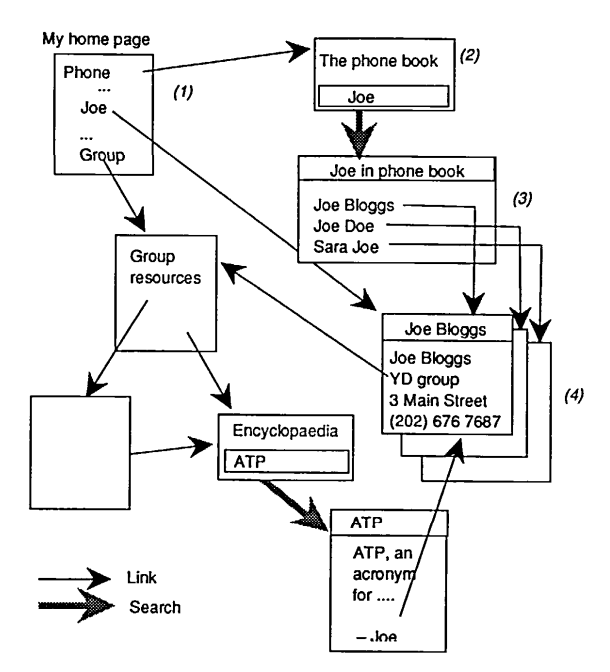
\includegraphics[width=\linewidth]{gambar/w3_model}
	\caption{Gambar sebuah web yang terdiri atas kumpulan \textit{link} dan indeks \citep{bernersLee1992}}
	\label{gambar:w3_model}
\end{figure}

Model yang dipakai WWW menggunakan dua paradigma dari \textit{hypertext link} dan pencarian teks yang saling melengkapi. Gambar \ref{gambar:w3_model} menunjukkan bagaimana sebuah web yang berisi informasi pribadi terbentuk pada paradigma ini. Pembaca mulai pada halaman \textit{home} (1) lalu menggunakan \textit{link} grup atau publik untuk mencari bahan informasi. Indeks seperti buku telepon (2) ditampilkan sebagai dokumen yang memungkinkan untuk melakukan input pencarian. Hasil dari pencarian berupa dokumen \textit{hypertext} virtual (3) yang menunjuk pada dokumen yang ditemukan (4) \citep{bernersLee1992}.

\subsection{Teori Graf}

\begin{figure}[!htb]
\begin{minipage}{0.48\linewidth}
	\centering
	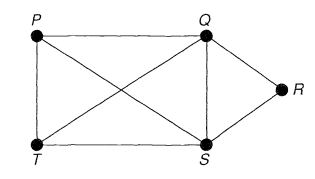
\includegraphics[width=.7\linewidth]{gambar/graph_example}
	\caption{Contoh graf \citep{wilson1996}}
	\label{gambar:graph_example}
\end{minipage}\hfill
\begin{minipage}{0.48\linewidth}
	\centering
	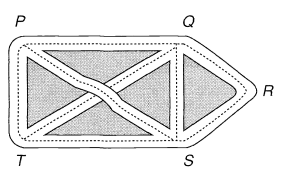
\includegraphics[width=.7\linewidth]{gambar/graph_example_2}
	\caption{Contoh peta jalan yang dapat diandaikan sebagai graf \citep{wilson1996}}
	\label{gambar:graph_example_2}
\end{minipage}
\end{figure}

\begin{figure}
	\centering
	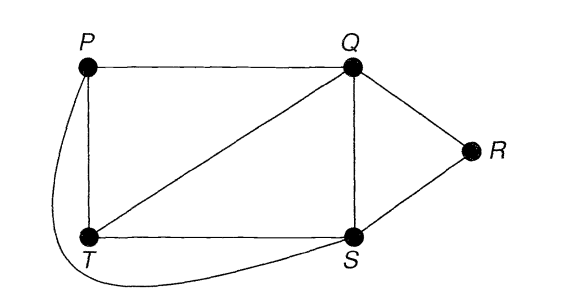
\includegraphics[keepaspectratio, width=0.48\linewidth]{gambar/graph_example_3}
	\caption{}
	\label{gambar:graph_example_3}
\end{figure}

Graf adalah sebuah representasi dari himpunan titik (\textit{node / vertice}) dan bagaimana titik-titik tersebut saling terhubung tanpa memperdulikan sifat metriknya \citep{wilson1996}. Pada gambar \ref{gambar:graph_example} merupakan contoh graf, dengan $P$, $Q$, $R$, $S$, $T$ merupakan titik, dan masing-masing terhubung dengan garis (\textit{edge}). Garis yang menghubungkan titik $P$ dan $S$ disebut dengan $PS$, sedangkan garis yang menghubungkan titik $Q$ dan $T$ disebut dengan $QT$. Persilangan antara $PS$ dan $QT$ tidak disebut sebagai titik, karena keduanya tidak saling bersilangan, melainkan saling melompati layaknya gambar \ref{gambar:graph_example_2}. Selanjutnya, kedua graf dianggap sama, jika dan hanya jika titik yang berkorespondensi sama-sama terhubung dengan garis yang sama dengan garis pada graf lainnya \citep{wilson1996}. Sebagai contoh, graf pada gambar \ref{gambar:graph_example_3} merupakan graf yang sama dengan graf pada gambar \ref{gambar:graph_example} \citep{wilson1996}. 

\begin{figure}[!htb]
\begin{minipage}{0.48\linewidth}
	\centering
	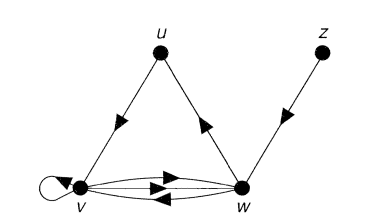
\includegraphics[width=.7\linewidth]{gambar/digraph_example}
	\caption{Contoh digraf \citep{wilson1996}}
	\label{gambar:digraph_example}
\end{minipage}\hfill
\begin{minipage}{0.48\linewidth}
	\centering
	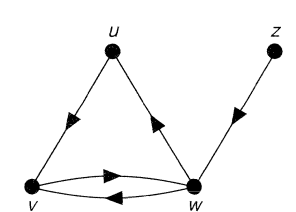
\includegraphics[width=.7\linewidth]{gambar/simple_digraph_example}
	\caption{Contoh digraf sederhana \citep{wilson1996}}
	\label{gambar:simple_digraph_example}
\end{minipage}
\end{figure}

Garis pada graf dapat diberikan arah. Garis pada graf yang berarah disebut sebagai busur (\textit{arc}). Graf yang memiliki arah pada garisnya disebut dengan graf berarah (\textit{directed graph / digraph} / digraf) yang terdiri atas himpunan titik dan busur \citep{wilson1996}. Pada digraf di gambar \ref{gambar:digraph_example} terdapat himpunan titik $u$, $v$, $w$, dan $z$, dengan busur $uv$, $vv$, $vw (2\times)$, $wv$, $wu$, dan $zw$. Sebuah digraf disebut sebagai digraf sederhana jika himpunan busurnya tidak ada yang sama (\textit{distinct}) dan tidak memiliki \textit{loop} (contoh: busur $vv$) \citep{wilson1996}. Digraf pada gambar \ref{gambar:simple_digraph_example} adalah contoh digraf sederhana.

\subsection{Pagerank}

Jika World Wide Web diibaratkan pada sebuah graf berarah, halaman web adalah titik graf, \textit{link} adalah garis. Lalu \textit{link} yang menunjuk keluar dari titik disebut \textit{forward link}, sedangkan \textit{link} yang menunjuk kedalam titik disebut \textit{backlink}. Sangat sulit untuk mengetahui semua \textit{backlink} suatu halaman web, tetapi sangat mudah untuk mengetahui semua \textit{forward link} suatu halaman web yaitu dengan cara mengunduh halaman web tersebut \citep{ilprints422}. Setiap halaman web memiliki jumlah \textit{backlink} yang beragam. Pada saat Pagerank diteliti, halaman \textit{home} NetScape memiliki 62.804 \textit{backlink} dibandingkan halaman web kebanyakan yang hanya memiliki beberapa \textit{backlink}. Secara umum suatu halaman web jika memiliki banyak \textit{backlink} dapat dianggap lebih penting daripada halaman web lain yang memiliki lebih sedikit \textit{backlink}. Perhitungan jumlah sitasi sederhana pernah digunakan untuk memprediksi pemenang Nobel masa depan \citep{ilprints422}. 

\begin{equation}
	\label{eq:5-1}
	P_{ij}= 
	\begin{cases}
		\frac{d}{C_j} + \frac{(1-d)}{N} & j \to i \\
		\frac{(1-d)}{N} & j \not\to i \text{ dan } C_j \not=0 \\
		\frac{1}{N} & C_j = 0
	\end{cases}
\end{equation}

Graf pada WWW, dapat direpresentasikan sebagai matriks transisi. Sebelumnya matriks transisi didefinisikan sebagai matriks $X$, berubah menjadi matriks $P$ sesuai dengan penelitian \citet{zhuetal2005distributedPagerank}. Matriks $P$ didefinisikan pada persamaan \ref{eq:5-1}. $C_j$ adalah jumlah \textit{forward link} dari halaman $j$. $j \to i$ adalah halaman $j$ memiliki \textit{link} menuju halaman $i$.

Selanjutnya algoritma Pagerank didefinisikan pada algoritma \ref{alg:1.1}

\begin{algorithm}
	\floatname{algorithm}{Algoritma}
	\caption{Pagerank \citep{zhuetal2005distributedPagerank}}
	\label{alg:1.1}
	\begin{algorithmic}[1]
		\State Definisikan $\pi^0$ awal-awal
		\State $k \gets 0$
		\State \label{alg:1.1.step:start_loop} $\pi^{\sim k+1} \gets P \pi^k$
		\State $\pi^{k+1} \gets \frac{\pi^{\sim k+1}}{||\pi^{\sim k+1}||_1}$
		\State Jika $||\pi^{k+1} - \pi^k|| < \epsilon$  berhenti dan kembalikan nilai $\pi^{k+1}$
		\State $k \gets k+1$
		\State Ulangi langkah \ref{alg:1.1.step:start_loop}
	\end{algorithmic}
\end{algorithm}

\subsection{Distributed Pagerank Computation (DPC)}

Jika \textit{link} pada kumpulan web dibuat kedalam graf, maka graf tersebut akan memiliki sebuah struktur menyerupai blok, karena mayoritas dari \textit{link} tersebut bersifat \textit{intra-host}, merujuk halaman yang masih di dalam \textit{host} yang sama. Oleh karena itu, jika dilakukan perjalanan acak pada kumpulan web tersebut dapat dilihat sebagai rantai Markov \textit{Nearly Completely Decomposable} (NCD) \citep{zhuetal2005distributedPagerank}. Rantai Markov NCD adalah rantai Markov yang dapat dipartisi sehingga peluang dari keadaan awal ke keadaan selanjutnya lebih sering menunjuk keadaan yang berada di dalam partisinya dibandingkan di luar partisinya \citep{kontovasilisMitrou1995}. Oleh karena itu, dasar dari algoritma DPC adalah mengelompokan halaman web berdasarkan domainnya \citep{zhuetal2005distributedPagerank}.

Masalah dari algoritma Pagerank biasa adalah besarnya memori utama yang dibutuhkan untuk bisa menyimpan matriks $X$ (lihat persamaan \ref{eq:2}). Oleh karena itu, dirumuskan algoritma Pagerank terdistribusi. DPC, dirumuskan oleh \citet{zhuetal2005distributedPagerank}, memakai mekanisme interaksi sederhana antara \textit{cluster} dan lalu lintas komunikasi rendah. Ditinjau dari perspektif matematika, dibuktikan bahwa algoritma DPC setara dengan metode \textit{Iterative Aggregation-Disaggregation} (IAD) dengan \textit{Block Jacobi smoothing}. DPC juga memiliki keunggulan dibandingkan dengan algoritma Pagerank biasa yaitu, matriks-matriks dipecah menjadi matriks agregasi dan matriks lokal sehingga ukurannya cukup kecil untuk disimpan di memori utama, sehingga mempercepat komputasi karena tiap iterasi memerlukan sedikit operasi I/O pada \textit{disk}. Selanjutnya, Vektor Pagerank lokal konvergen lebih cepat pada beberapa \textit{cluster} tertentu, berbeda dengan Pagerank biasa karena terdapat komputasi tidak perlu pada \textit{cluster} yang sudah konvergen \citep{zhuetal2005distributedPagerank}.

Sebelum langsung membahas algoritma DPC, akan didefinisikan beberapa notasi terlebih dahulu. $e=(1,...,1)^T$. Misal G adalah himpunan bilangan bulat $\{1,...,N\}$. Misal $G_1,...G_n, n \leq N$ adalah grup agregasi dari elemen-elemen di $G$. Himpunan-himpunan $G_i, i = 1,...,n$, adalah saling lepas dan $\cup^n_{i=1}G_i=G$. Misal $N_i$ adalah ordo dari himpunan $G_i$, atau jumlah elemen-elemen di $G_i$ \citep{zhuetal2005distributedPagerank}. 

Misal $R$ adalah matriks agregasi $n \times N$, yang memenuhi persamaan \ref{eq:3} \citep{zhuetal2005distributedPagerank}.

\begin{equation}
	\label{eq:3}
	R_{ij}= 
	\begin{cases}
			1 & j \in G_i\\
			0 & \text{lainnya}
	\end{cases}
\end{equation}

Dilakukan partisi pada vektor positif $\pi$ menjadi $(\pi^T_1,\pi^T_2,...,\pi^T_n)^T$ berdasarkan $\{G_i\}$. $\pi_i$ adalah subvektor dengan dimensi $N_i$ \citep{zhuetal2005distributedPagerank}.

Maka dapat didefinisikan matriks disagregasi $S(\pi)$ $N \times n$ sebagai persamaan \ref{eq:4} \citep{zhuetal2005distributedPagerank}.
\begin{equation}
	\label{eq:4}
	S(\pi) = 
	\begin{pmatrix}
		S(\pi)_1 & 0 & \ldots & 0 \\
		0 & S(\pi)_2 & \ldots & 0 \\
		\vdots & \vdots & \ddots & \vdots \\
		0 & 0 & \ldots & S(\pi)_n
	\end{pmatrix}
\end{equation}
Dimana $S(\pi)_i$ adalah sebuah kolom vektor yang mewakili \textit{censored stationary distribution} dari halaman-halaman di \textit{cluster} $G_i$. Ingat bahwa $RS(\pi) = I$ \citep{zhuetal2005distributedPagerank}.

Matriks transisi $P$ dipartisi menjadi beberapa blok berdasarkan $\{G_i\}$ menjadi seperti persamaan \ref{eq:6} \citep{zhuetal2005distributedPagerank}.
\begin{equation}
\label{eq:6}
	P =
	\begin{pmatrix}
		P_{11} & P_{12} & \ldots & P_{1n} \\
		P_{21} & P_{22} & \ldots & P_{2n} \\
		\vdots & \vdots & \ddots & \vdots \\
		P_{n1} & P_{n2} & \ldots & P_{nn}
	\end{pmatrix}
\end{equation}
Dilambangkan blok baris ke-$i$ sebagai persamaan \ref{eq:7}
\begin{equation}
\label{eq:7}
	P_{i*} \overset{\Delta}{=} (P_{i1},\ldots,P_{in})
\end{equation}
dan dilambangkan blok kolom ke-$i$ sebagai persamaan \ref{eq:8}
\begin{equation}
\label{eq:8}
	P_{*i} \overset{\Delta}{=}
	\begin{pmatrix}
		P_{1i} \\
		\vdots \\
		P_{ni} 
	\end{pmatrix}
\end{equation} 

Setiap blok diagonal $P_{ii}$ adalah matriks persegi dan merupakan matriks \textit{intra-cluster} \textit{link} dari \textit{cluster} $G_i$, sementara blok-blok di luar diagonal merupakan struktur \textit{link} antar-\textit{cluster}. Selanjutnya, matriks agregat $A = RPS(\pi)$ adalah matriks transisi antar \textit{cluster}. Maka dapat dibuat algoritma DPC pada algoritma \ref{alg:3} \citep{zhuetal2005distributedPagerank}.

\begin{algorithm}
	\floatname{algorithm}{Algoritma}
	\caption{Algoritma DPC \citep{zhuetal2005distributedPagerank}}
	\label{alg:3}
	\begin{algorithmic}[1]
		\State Buat matriks transisi lokal untuk tiap \textit{cluster} $G_i$ berdasarkan $P$ 
			\begin{equation*} Q_i = LocalTransitionMatrix(G_i) \forall G_i \in G \end{equation*}
		\State $\pi_i^0 = Pagerank(Q_i, \frac{e}{N_i}, \epsilon) \forall G_i \in G$
		\State Inisialisasi $k = 0$
		\State \label{alg:3:step_rps}
			$A^k = RPS(\pi^k)$
		\State
			$z^k = Pagerank(A^k, \frac{e}{n}, \epsilon)$
		\State $\forall G_i \in G$ buat sebuah \textit{extended local transition matrix} $(N_i + 1) \times (N_i + 1)$. Dimana skalar $\alpha^k$ membuat jumlah nilai kolom dari $B^k_i$ adalah satu
			\begin{equation*}
				B_i^k =
				\begin{pmatrix}
					P_{ii} 		& \frac{(P_{i*}S(\pi^k)z^k - P_{ii}\pi_i^kz_i)}{(1 - z^k_i)} \\
					e^TP_{*i} & \alpha^k
				\end{pmatrix}
			\end{equation*}
		\State Hitung vektor \textit{extended local Pagerank}. Dimana $\beta^{k+1}_i$ adalah skalar
			\begin{equation*}
				\begin{pmatrix}
					\omega^{k+1}_i \\
					\beta^{k+1}_i
				\end{pmatrix}
				= Pagerank(B^k_i, \frac{e}{(N_i + 1)}, \epsilon)
			\end{equation*}
		\State $\pi^{\sim k+1}_i = \frac{1 - z^k_i}{\beta^{k+1}_i} \omega^{k+1}_i$
		\State $\pi^{k+1} = \frac{\pi^{\sim k+1}}{||\pi^{\sim k+1}||_1}$
		\State $k = k+1$
		\State Jika $||\pi^{k+1} - \pi^k|| < \epsilon$ terpenuhi, berhenti dan berikan $\pi^{k}$ sebagai hasil akhir. Jika sebaliknya, kembali ke langkah \ref{alg:3:step_rps}
	\end{algorithmic}
\end{algorithm}

%------------------------------------------------

\section{III. METODOLOGI}

\subsection{Tahapan Penelitian}

Terdapat tahapan-tahapan yang harus dilalui untuk melaksanakan penelitian ini. Tahapan penelitian dapat dilihat pada diagram \ref{gambar:tahapan_penelitian}. Terdapat beberapa algoritma yang belum dijelaskan sebelumnya seperti Modified DPC (MDPC) dan Random Walker. Algoritma MDPC dirumuskan karena kekurangan dari algoritma DPC yang akan dijelaskan pada bagian selanjutnya. Sedangkan algoritma Random Walker merupakan program yang mensimulasikan pergerakan kunjungan halaman web dan merupakan basis dari algoritma Pagerank \citep{ilprints422}, sehingga sangat cocok untuk dijadikan sebagai acuan untuk melakukan verifikasi hasil.

\begin{figure}
	\centering
	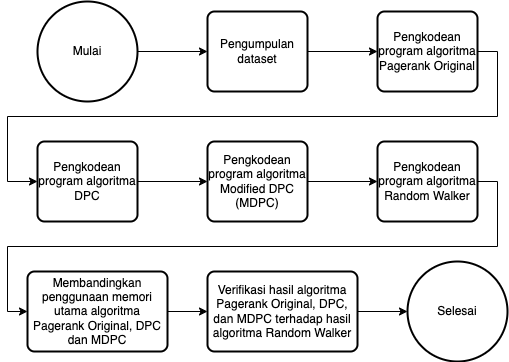
\includegraphics[keepaspectratio, width=\linewidth]{gambar/tahapan_penelitian.png}
	\caption{Diagram tahapan penelitian}
	\label{gambar:tahapan_penelitian}
\end{figure}

\subsection{Pengumpulan Dataset}

Pada penelitian ini digunakan dua \textit{dataset}. \textit{Dataset} pertama yang nantinya disebut sebagai Dataset 1 merupakan \textit{dataset} yang diperoleh dengan cara \textit{crawling}. Memiliki 20.493 baris halaman web \textit{page\_information} dan 2.915.842 baris \textit{page\_linking}. Data \textit{page\_information} pada Dataset 1 dapat dikelompokan ke dalam 560 \textit{cluster} berdasarkan \textit{domain}-nya yang dapat dilihat pada tabel \ref{domain:dataset1}.

\begin{table}
	\centering
	\caption{Data \textit{cluster} pada Dataset 1. Simbol "-" merupakan potongan nama domain karena terlalu panjang}
	\label{domain:dataset1}
	\begin{tabular}{|c|c|c|}
	\hline
	\textbf{Domain} & \textbf{Halaman} \\
	\hline
	detik.com & 2.215 \\
	unj.ac.id & 2.208 \\
	sport.detik.com & 1.279 \\
	finance.detik.com & 1.098 \\
	repository.unj.ac.id & 1.089 \\
	news.detik.com & 802 \\
	oto.detik.com & 779 \\
	inet.detik.com & 671 \\
	support.google.com & 630 \\
	food.detik.com & 626 \\
	\vdots & \vdots \\
	-competitions.withgoogle.com & 1 \\
	googledevelopers.blogspot.com & 1 \\
	skillshop.exceedlms.com & 1 \\
	\hline
	\end{tabular}
\end{table}

Yang kedua, Dataset 2 merupakan \textit{dataset} kecil dan \textit{domain} kecil yang sengaja dikumpulkan untuk melihat perbedaan performa algoritma antara \textit{dataset} yang berisi banyak \textit{domain} besar dengan \textit{dataset} yang berisi \textit{domain} kecil. Batasan pada tiap \textit{domain} yang dipakai ketika mengumpulkan data adalah 20 halaman web per \textit{domain}. Pada Dataset 2 terdapat 100 baris \textit{page\_information}, 5.944 baris \textit{page\_linking}, serta 5 \textit{cluster} atau \textit{domain}. Data \textit{cluster} pada Dataset 2 dapat dilihat pada tabel \ref{domain:dataset2}.

\begin{table}
	\centering
	\caption{Data \textit{cluster} pada Dataset 2}
	\label{domain:dataset2}
	\begin{tabular}{|c|c|}
	\hline
	\textbf{Domain} & \textbf{Halaman} \\
	\hline
	unj.ac.id & 20 \\
	ppid.unj.ac.id & 20 \\
	fip.unj.ac.id & 20 \\
	fbs.unj.ac.id & 20 \\
	fmipa.unj.ac.id & 20 \\
	\hline
	\end{tabular}
\end{table}

\subsection{Algoritma Modified DPC}

Diusulkan algoritma modifikasi dari algoritma DPC atau Modified DPC (MDPC). Secara garis besar MDPC hanya memangkas langkah-langkah pada algoritma DPC, berdasarkan gagasan utama DPC yaitu melakukan perhitungan terpisah \textit{ranking} halaman web berdasarkan \textit{domain}-nya, dan melakukan perhitungan penggabungan dengan menghitung \textit{ranking} \textit{domain} itu sendiri. Masalah utama dari algoritma DPC adalah langkah memperoleh matriks $A$ pada langkah \ref{alg:3:step_rps} yang melakukan perkalian matriks $P$ secara utuh.

Definisi matriks $A$ versi MDPC yang selanjutnya akan berganti notasi menjadi $A_{mdpc}$ dapat dilihat pada persamaan \ref{eq:a_mdpc}. Makna notasi $P_{**}$ merupakan partisi matriks transisi $P$ yang sudah didefinisikan pada persamaan \ref{eq:6}, sedangkan makna dari \textit{sum} adalah nilai total dari elemen matriks.

\begin{equation}
	\label{eq:a_mdpc}
	A_{mdpc} =
	\begin{pmatrix}
		\frac{\text{sum}(P_{11})}{\text{sum}(P_{*1})} & \cdots & \frac{\text{sum}(P_{1i})}{\text{sum}(P_{*i})} \\
		\vdots & \ddots & \vdots \\
		\frac{\text{sum}(P_{i1})}{\text{sum}(P_{*1})} & \cdots & \frac{\text{sum}(P_{ii})}{\text{sum}(P_{*i})}
	\end{pmatrix}
\end{equation}

Langkah-langkah algoritma MDPC dapat dilihat pada algoritma \ref{alg:mdpc}.

\begin{algorithm}
	\floatname{algorithm}{Algoritma}
	\caption{Algoritma MDPC}
	\label{alg:mdpc}
	\begin{algorithmic}[1]
		\State Buat matriks transisi lokal $N_i \times N_i$ untuk tiap \textit{cluster} $G_i$ berdasarkan $P$ 
			\begin{equation*} Q_i = LocalTransitionMatrix(G_i) \forall G_i \in G \end{equation*}
		\State $\pi_i = Pagerank(Q_i, \frac{e}{N_i}, \epsilon) \forall G_i \in G$
		\State $z = Pagerank(A_{mdpc}, \frac{e}{n}, \epsilon)$
		\State $\pi_i \gets \pi_i \times z_i \forall i \in 1 \ldots n$
		\State kembalikan $\pi$ sebagai hasil akhir. $\pi$ adalah vektor gabungan $N \times 1$ dari semua $\pi_i$.
	\end{algorithmic}
\end{algorithm}

\subsection{Algoritma Random Walker}

Basis intiutif dari algoritma Pagerank adalah \textit{random walk} pada graf. Versi penyederhanaan dalam bentuk distribusi probabilitas \textit{random walk} pada sebuah graf web \citep{ilprints422}. Akan dibuat sebuah program yang mensimulasikan dari proses \textit{random walk} ini yang disebut Algoritma Random Walker. Algoritma Random Walker dipakai untuk membandingkan hasil perhitungan algoritma DPC, MDPC, dan Pagerank asli. Langkah-langkah pada Algoritma Random Walker dapat dilihat pada algoritma \ref{alg:random_walker}.

\begin{algorithm}
	\floatname{algorithm}{Algoritma}
	\caption{Algoritma Random Walker}
	\label{alg:random_walker}
	\begin{algorithmic}[1]
		\State Tentukan jumlah iterasi dan jumlah $walker$ awal-awal pada setiap halaman web
		\State Instansiasi $walker$ sama banyak pada setiap halaman web
		\State Bentuk matriks $P$ sesuai persamaan \ref{eq:5-1}
		\State Untuk setiap $walker$, pindahkan $walker$ ke halaman web selanjutnya berdasarkan peluang $P_{*i}$, untuk $i$ adalah indeks halaman web $walker$ saat ini.
		\State Ulangi langkah 4 sebanyak jumlah iterasi. \textit{Ranking} halaman web ditentukan pada banyaknya jumlah $walker$ yang tinggal.
	\end{algorithmic}
\end{algorithm}

Pada penelitian ini, algoritma Random Walker tidak dipakai untuk membandingkan performa, melainkan sebatas pembanding hasil dari algoritma Pagerank, DPC, dan MDPC.

\subsection{Tahapan Pengembangan}

Akan dilakukan pengkajian efisiensi penggunaan memori utama pada algoritma Pagerank, DPC, dan MDPC. Penelitian ini merupakan sub-penelitian dari penelitian utama tentang pengembangan \textit{search engine}. Telah dilakukan penelitian sebelumnya oleh \citet{qoriiba2021perancangan} yang membuat modul \textit{crawler} dan modul pendukung lain. Selanjutnya \citet{khatulistiwa2022SearchEngine} menggabungkan modul \textit{crawler} \citet{qoriiba2021perancangan}, Google Pagerank, dan \textit{searcher} berbasis TF IDF menjadi \textit{search engine} berbasis konsol. Di saat yang berdekatan, \citet{pratama2022indexer} membuat modul \textit{indexer} menggunakan \textit{Induced Generalized Suffix Tree} dan \citet{zalghornain2022indexer} menggunakan \textit{Continuous-Bag-of-Words} dan Model \textit{Continuous Skip-Gram}. 

Karena penelitian ini merupakan sub-penelitian, maka \textit{stack} teknologi yang digunakan dalam implementasi penelitian ini akan disamakan dengan penelitian induk yaitu menggunakan bahasa pemrograman Python 3 dan basis data MySQL. Implementasi algoritma akan mengikuti algoritma-algoritma yang sudah dijelaskan sebelumnya. Perkiraan pengerjaan adalah satu bulan, dan tidak menutup kemungkinan akan memakan waktu lebih lama atau lebih cepat tergantung kesulitan dan kompleksitas yang dihadapi.

Untuk menguji penggunaan memori, waktu eksekusi, dan hasil algoritma \textit{ranking} halaman web maka dilakukan langkah-langkah berikut:
\begin{enumerate}
	\item{Dilakukan pengkodean empat program algoritma yaitu Pagerank Original, DPC, MDPC, dan Random Walker}
	\item{Ditentukan nilai masukan \textit{damping factor}, toleransi \textit{error}, serta dataset yang sama}
	\item{Jalankan program Pagerank Original, DPC, MDPC, dan Random Walker terhadap dataset 1 (20.493 Halaman)}
	\item{Bandingkan lamanya waktu, dan penggunaan memori utama algoritma Pagerank Original, DPC, dan MDPC}
	\item{Verifikasi kemiripan hasil antara algoritma Pagerank Original, DPC, dan MDPC terhadap algoritma Random Walker}
	\item{Jalankan program Pagerank Original, DPC, MDPC, dan Random Walker terhadap dataset 2 (100 Halaman)}
	\item{Bandingkan lamanya waktu, dan penggunaan memori utama algoritma Pagerank Original, DPC, dan MDPC}
	\item{Verifikasi kemiripan hasil antara algoritma Pagerank Original, DPC, dan MDPC terhadap algoritma Random Walker}
\end{enumerate}

\subsection{Metode Perbandingan}

Terdapat tiga hal yang dibandingkan pada penelitian ini, yang pertama adalah perbandingan penggunaan memori utama, lama waktunya algoritma dijalankan, dan kemiripan hasil yang dikeluarkan oleh ketiga algoritma. Tidak ada metode khusus untuk membandingkan penggunaan memori utama, dan lama waktu eksekusi. Ketiga algoritma hanya dijalankan lalu dapat dilihat dan dibandingkan penggunaan memori utama dan lamanya waktu eksekusi tiap algoritma. Sedangkan untuk kemiripan hasil, penelitian ini mengikuti metode yang dipakai oleh \citet{zhuetal2005distributedPagerank}, digunakan perhitungan jarak \textit{Kendall's $\tau$} atau dapat disebut sebagai $KDist$.

Rumus dari jarak $KDist$ antara vektor \textit{ranking} halaman web $\pi$ terhadap $\hat{\pi}$ secara berurutan dapat dilihat pada persamaan \ref{eq:kendall_distance}, di mana $0 \leq KDist(\pi, \hat{\pi}) \leq 1$. Semakin kecil nilai jaraknya maka dianggap lebih mirip.

\begin{equation}
	K_{ij}(\pi, \hat{\pi}) = 
	\begin{cases}
		1 & \pi_i \geq \pi_j \text{ and } \hat{\pi}_i < \hat{\pi}_j \\
		1 & \pi_i < \pi_j \text{ and } \hat{\pi}_i \geq \hat{\pi}_j \\
		0 & \text{lainnya}
	\end{cases}
\end{equation}

\begin{equation}
	\label{eq:kendall_distance}
	KDist(\pi, \hat{\pi}) = \frac{\Sigma_{1 \leq i < j \leq N} K_{ij}(\pi, \hat{\pi})}{\frac{1}{2} N(N-1)}
\end{equation}

%------------------------------------------------

\section{IV. Hasil}

Setelah program berhasil dibuat dan dijalankan terhadap semua \textit{dataset}, maka diperoleh hasil berikut. Pada Dataset 2 puncak penggunaan memori pada ketiga algoritma relatif sama, hal ini dikarenakan data yang cukup kecil dibandingkan \textit{overhead} memory pada program. Selanjutnya pada Dataset 1 puncak penggunaan memori terbesar ada pada algoritma pagerank asli yaitu sebesar 3,4 GB dimulai saat matriks $20.493\times 20.493$ $P$ dibentuk. Dengan perhitungan setiap sel matriks merupakan angka desimal \textit{floating point} 64bit maka besarnya matriks $P$ pada memori adalah $\pm$3,4 GB. 

Selanjutnya, pada algoritma DPC penggunaan memori terbesar adalah 842 MB yang terjadi pada pembentukan dan penyimpanan matriks $P_{*i}$ ke \textit{cache}. Mengingat domain terbesar di Dataset 1 yaitu "detik.com" dengan jumlah 2.215 halaman, maka dimensi matriks $P_{*i}$ terbesar adalah $20.493 \times 2.215$ yang akan memakan memori sebesar $\pm363$ MB, dan ketika akan disimpan ke dalam \textit{cache} menggunakan \textit{pickle library} akan dilakukan penyalinan objek sebelum ditulis ke dalam \textit{cache}, sehingga penggunaan memori $2 \times \pm363 MB = \pm726 MB$. 

Pada algoritma MDPC puncak memori sebesar $\pm86$ MB, penggunaan memori puncak terjadi pada langkah pembentukan dan penyimpanan matriks $Q$ ke \textit{cache}. Karena matriks $Q$ adalah matriks transisi lokal suatu domain, maka matriks $Q$ terbesar adalah matriks $Q$ domain "detik.com" dengan 2.215 halaman. Ukuran matriks $Q$ yang terbentuk adalah $2.215 \times 2.215$ yang secara ukuran di memori adalah $\pm39$ MB, dan di tengah proses penyimpanan ke dalam \textit{cache} dilakukan penyalinan objek sementara, sehingga ukuran memorinya menjadi dua kali lipat yaitu $\pm86$ MB. Perbandingan puncak memori dan lamanya waktu eksekusi algoritma Pagerank Original, algoritma Distributed Pagerank Computation (DPC), dan algoritma Modified DPC (MDPC), dapat dilihat pada tabel \ref{table:algorithm_performance}.

\begin{table}
	\caption{Puncak penggunaan memori (dalam \textit{Mega Byte}) dan waktu eksekusi (dalam detik)}
	\label{table:algorithm_performance}
	\begin{tabular}{|c|c|c|}
		\hline
		\textbf{Algoritma} & \textbf{Puncak Memori} & \textbf{Waktu} \\
		\hline
		\multicolumn{3}{|c|}{Dataset 1} \\
		\hline
		PR & 3.417,632 & 328,803 \\
		DPC & 842,482 & 1.151,628 \\
		MDPC & 86,582 & 816,375 \\
		\hline
		\multicolumn{3}{|c|}{Dataset 2} \\
		\hline
		PR & 2,045 & 0,568 \\
		DPC & 2,056 & 19,372 \\
		MDPC & 2,055 & 0,652 \\
		\hline
	\end{tabular}
\end{table}

Selanjutnya akan dihitung nilai kemiripan antara nilai Pagerank yang dihasilkan program Pagerank asli, DPC, MDPC, dan Random Walker. Nilai Pagerank berbentuk vektor dan diurutkan berdasarkan \textit{id} halaman. Pada Dataset 1, nilai $KDist$ tiap vektor \textit{ranking} halaman web yang dihasilkan oleh algoritma Pagerank, DPC, MDPC, dan Random Walker dapat dilihat pada tabel \ref{table:kendall_distance_score_dataset_1}. 

\begin{table}
	\caption{Nilai jarak Kendall vektor Pagerank pada dataset 1 (20.493 halaman). Ket: Pagerank asli (PR), Random Walker (RW).}
	\label{table:kendall_distance_score_dataset_1}
	\begin{tabular}{|c|c|c|c|c|}
		\hline
		& \textbf{PR} & \textbf{DPC} & \textbf{MDPC} & \textbf{RW} \\
		\hline
		\textbf{PR} & 0,0 & 0,250 & 0,260 & 0,027 \\
		\hline
		\textbf{DPC} & 0,250 & 0,0 & 0,277 & 0,252 \\
		\hline
		\textbf{MDPC} & 0,260 & 0,277 & 0,0 & 0,264 \\
		\hline
		\textbf{RW} & 0,027 & 0,252 & 0,264 & 0,0 \\
		\hline
	\end{tabular}
\end{table}

Vektor yang paling mirip atau memiliki nilai $KDist$ terkecil adalah vektor Pagerank dan Random Walker yaitu sebesar $0,02716$ atau $2,7$ persen perbedaan urutan. Sedangkan $KDist$ untuk DPC terhadap Pagerank dan Random Walker secara berurutan adalah $0,24956$ dan $0,25208$ atau $25$ persen dan $25,2$ persen perbedaan urutan. Selanjutnya untuk $KDist$ MDPC terhadap DPC, Pagerank, dan Random Walker secara berurutan adalah $0,27681$, $0,25985$, dan $0,26387$ atau $27,7$ persen, $26$ persen, dan $26,4$ persen perbedaan urutan.

Pada Dataset 2, nilai $KDist$ tiap vektor \textit{ranking} halaman web yang dihasilkan oleh algoritma Pagerank, DPC, MDPC, dan Random Walker dapat dilihat pada tabel \ref{table:kendall_distance_score_dataset_2}. Vektor yang paling mirip atau memiliki nilai $KDist$ terkecil adalah vektor Pagerank dan Random Walker yaitu sebesar $0,03293$ atau $3,3$ persen perbedaan urutan. Sedangkan $KDist$ untuk DPC terhadap Pagerank dan Random Walker secara berurutan adalah $0,17131$ dan $0,19131$ atau $17,1$ persen dan $19,1$ persen perbedaan urutan. Selanjutnya untuk $KDist$ MDPC terhadap DPC, Pagerank, dan Random Walker secara berurutan adalah $0,11091$, $0,12586$, dan $0,14949$ atau $11,1$ persen, $12,6$ persen, dan $14,9$ persen perbedaan urutan.

\begin{table}
	\caption{Nilai jarak Kendall vektor Pagerank pada dataset 2 (100 halaman). Ket: Pagerank asli (PR), Random Walker (RW).}
	\label{table:kendall_distance_score_dataset_2}
	\begin{tabular}{|c|c|c|c|c|}
		\hline
		& \textbf{PR} & \textbf{DPC} & \textbf{MDPC} & \textbf{RW} \\
		\hline
		\textbf{PR} & 0,0 & 0,171 & 0,126 & 0,033 \\
		\hline
		\textbf{DPC} & 0,171 & 0,0 & 0,111 & 0,191 \\
		\hline
		\textbf{MDPC} & 0,126 & 0,111 & 0,0 & 0,149 \\
		\hline
		\textbf{RW} & 0,033 & 0,191 & 0,149 & 0,0 \\
		\hline
	\end{tabular}
\end{table}

Perbedaan hasil cukup signifikan antara Distributed Pagerank Computation (DPC) dan Modified DPC (MDPC) terhadap Pagerank Original dan Random Walker disebabkan karena dasar dari perhitungannya yang berbeda. DPC dan MDPC memisahkan halaman web berdasarkan domain-nya, sedangkan Pagerank dan Random Walker melakukan perhitungan secara utuh.

Dapat disimpulkan, algoritma Pagerank Original paling cepat dan paling mirip hasilnya dengan algoritma Random Walker dalam melakukan pe-\textit{ranking}-an halaman web, namun memerlukan memori utama yang lebih besar. Sedangkan algoritma DPC dan MDPC memerlukan memori utama lebih kecil, sehingga cocok untuk komputer satu mesin dengan memori utama terbatas, tetapi dengan konsekuensi perbedaan hasil yang cukup besar terhadap algoritma Pagerank Original dan algoritma Random Walker dan waktu eksekusi yang lebih lambat.

%----------------------------------------------------------------------------------------

\section{V. KESIMPULAN DAN SARAN}

\subsection{Kesimpulan}
Berdasarkan hasil implementasi dan pengujian program Algoritma Pagerank, DPC, MDPC, dan Random Walker, maka diperoleh kesimpulan sebagai berikut:

\begin{enumerate}
	\item Algoritma Pagerank merupakan algoritma untuk menghitung \textit{ranking} halaman web yang berbasis pada Random Walk di graf halaman web \citep{ilprints422}. Algoritma Pagerank memiliki masalah pada penggunaan memori yang besar. Algoritma DPC yang memakai metode \textit{divide and conquer} \citep{zhuetal2005distributedPagerank} dipakai untuk menjawab permasalahan pada algoritma Pagerank. Algoritma MDPC merupakan modifikasi dari algoritma DPC yang dirumuskan pada penelitian ini karena terdapat langkah-langkah yang bisa disederhanakan pada algoritma DPC. Program simulasi Random Walker dibuat untuk menjadi pembanding dari hasil algoritma Pagerank, DPC, dan MDPC.
	
	\item Dari hasil pengujian algoritma pe-\textit{ranking}-an halaman web tercepat dalam waktu eksekusi dipegang oleh algoritma Pagerank, sedangkan dari segi penggunaan memori puncak, MDPC dan DPC jauh lebih kecil dibandingkan algoritma Pagerank. Walaupun demikian, setelah dilakukan uji hasil \textit{ranking} dengan menghitung nilai $KDist$ antara masing-masing algoritma, hasil dari algoritma Pagerank sangat mirip dengan hasil dari algoritma Random Walker dibandingan dengan algoritma DPC, dan MDPC terhadap Random Walker. Sehingga dapat disimpulkan algoritma DPC dan MDPC cocok untuk komputer satu mesin dengan memori utama terbatas, tetapi dengan mengorbankan kemiripan hasil dan waktu eksekusi lebih lambat.
\end{enumerate}

\subsection{Saran}
Adapun saran untuk penelitian selanjutnya adalah:
\begin{enumerate} 
	\item Menguji keempat algoritma lebih lanjut dengan dataset yang lebih besar dan beragam
    \item Mencari algoritma alternatif lain dari Pagerank yang secara performa memori dan waktu lebih baik, tetapi perbedaan hasil \textit{ranking} di bawah 10 persen
\end{enumerate}

%----------------------------------------------------------------------------------------
%	 REFERENCES
%----------------------------------------------------------------------------------------
\bibliography{daftar-pustaka}
\bibliographystyle{myapalike}
%----------------------------------------------------------------------------------------

\end{document}
